\documentclass[journal=jacsat,manuscript=article]{achemso}

%%%%%%%%%%%%%%%%%%%%%%%%%%%%%%%%%%%%%%%%%%%%%%%%%%%%%%%%%%%%%%%%%%%%%
%% Place any additional packages needed here.  Only include packages
%% which are essential, to avoid problems later. Do NOT use any
%% packages which require e-TeX (for example etoolbox): the e-TeX
%% extensions are not currently available on the ACS conversion
%% servers.
%%%%%%%%%%%%%%%%%%%%%%%%%%%%%%%%%%%%%%%%%%%%%%%%%%%%%%%%%%%%%%%%%%%%%
\usepackage[version=3]{mhchem} % Formula subscripts using \ce{}

%%%%%%%%%%%%%%%%%%%%%%%%%%%%%%%%%%%%%%%%%%%%%%%%%%%%%%%%%%%%%%%%%%%%%
%% If issues arise when submitting your manuscript, you may want to
%% un-comment the next line.  This provides information on the
%% version of every file you have used.
%%%%%%%%%%%%%%%%%%%%%%%%%%%%%%%%%%%%%%%%%%%%%%%%%%%%%%%%%%%%%%%%%%%%%
%%\listfiles

%%%%%%%%%%%%%%%%%%%%%%%%%%%%%%%%%%%%%%%%%%%%%%%%%%%%%%%%%%%%%%%%%%%%%
%% Place any additional macros here.  Please use \newcommand* where
%% possible, and avoid layout-changing macros (which are not used
%% when typesetting).
%%%%%%%%%%%%%%%%%%%%%%%%%%%%%%%%%%%%%%%%%%%%%%%%%%%%%%%%%%%%%%%%%%%%%
\newcommand*\mycommand[1]{\texttt{\emph{#1}}}
\newcommand{\bfv}[1]{{\mbox{\boldmath{$#1$}}}}
\newcommand{\x}{\bfv{x}}
%%%%%%%%%%%%%%%%%%%%%%%%%%%%%%%%%%%%%%%%%%%%%%%%%%%%%%%%%%%%%%%%%%%%%
%% Meta-data block
%% ---------------
%% Each author should be given as a separate \author command.
%%
%% Corresponding authors should have an e-mail given after the author
%% name as an \email command. Phone and fax numbers can be given
%% using \phone and \fax, respectively; this information is optional.
%%
%% The affiliation of authors is given after the authors; each
%% \affiliation command applies to all preceding authors not already
%% assigned an affiliation.
%%
%% The affiliation takes an option argument for the short name.  This
%% will typically be something like "University of Somewhere".
%%
%% The \altaffiliation macro should be used for new address, etc.
%% On the other hand, \alsoaffiliation is used on a per author basis
%% when authors are associated with multiple institutions.
%%%%%%%%%%%%%%%%%%%%%%%%%%%%%%%%%%%%%%%%%%%%%%%%%%%%%%%%%%%%%%%%%%%%%
\author{Wei-Tse Hsu}
\author{Pascal T. Merz}
\affiliation{Department of Chemical and Biological Engineering, University of Colorado Boulder, Boulder, CO 80305}
\author{Giovanni Bussi}
\affiliation{Scuola Internazionale Superiore di Studi Avanzati, Trieste, Italy}
\author{Michael R. Shirts}
\affiliation{Department of Chemical and Biological Engineering, University of Colorado Boulder, Boulder, CO 80305}
\email{michael.shirts@colorado.edu}

%%%%%%%%%%%%%%%%%%%%%%%%%%%%%%%%%%%%%%%%%%%%%%%%%%%%%%%%%%%%%%%%%%%%%
%% The document title should be given as usual. Some journals require
%% a running title from the author: this should be supplied as an
%% optional argument to \title.
%%%%%%%%%%%%%%%%%%%%%%%%%%%%%%%%%%%%%%%%%%%%%%%%%%%%%%%%%%%%%%%%%%%%%
\title
  {Supporting Information: Adding alchemical variables to metadynamics to enhance sampling in free energy calculations}

%%%%%%%%%%%%%%%%%%%%%%%%%%%%%%%%%%%%%%%%%%%%%%%%%%%%%%%%%%%%%%%%%%%%%
%% Some journals require a list of abbreviations or keywords to be
%% supplied. These should be set up here, and will be printed after
%% the title and author information, if needed.
%%%%%%%%%%%%%%%%%%%%%%%%%%%%%%%%%%%%%%%%%%%%%%%%%%%%%%%%%%%%%%%%%%%%%
% \abbreviations{IR,NMR,UV}
%\keywords{American Chemical Society, \LaTeX}

%%%%%%%%%%%%%%%%%%%%%%%%%%%%%%%%%%%%%%%%%%%%%%%%%%%%%%%%%%%%%%%%%%%%%
%% The manuscript does not need to include \maketitle, which is
%% executed automatically.
%%%%%%%%%%%%%%%%%%%%%%%%%%%%%%%%%%%%%%%%%%%%%%%%%%%%%%%%%%%%%%%%%%%%%
\begin{document}

\section{Pair correlation function of the uncoupled state}
To calculate binding free energies corresponding to the standard concentration, we usually need to consider a correction term that accounts for the difference between the effective box volume in the uncoupled state and the molecular volume. While the effective box volume could be hard to estimate, this correction term can be incorporated in $\Delta A^{\text{complex}}_{\text{(restr)}_{\text{on}}}$, the free energy change upon the imposition of the restraint between the host and guest molecules in the complex simulation, which can be calculated analytically (assuming a harmonic restraint):
\begin{equation}
    \Delta A^{\text{complex}}_{\text{(restr)}_{\text{on}}} = k_{\text{B}}T\ln\left[\frac{3}{V_0}\left(\frac{\pi k_{\text{B}}T}{K}\right)^{3/2}\right]
\end{equation} where $K$ is the spring constant and $V_0$ is the molecular volume (1.6605 nm$^{3}$) that corresponds to 1 mol/L reference concentration. In a complex simulation where such a restraint is absent, however, we can only calculate the box volume correction term $\Delta A_{\text{corr}}$ as below by assuming that the effective box volume sampled by the ligand is equal to the box volume, i.e. the ligand was able to sample the entire simulation box:
\begin{equation}
    \Delta A_{\text{corr}}=-kT \ln\left(\frac{V_{\text{box}}}{V_0}\right)
\end{equation} where $V_{\text{box}}$ is the box volume. 

To examine whether the assumption was valid in the complex simulation of System 3, for both 1D and 2D alchemical metadynamics, we plotted the distributions of the COM distance between the host and guest molecules and compared them to the reference, which is an approximation to the real distribution assuming that the entire box was sampled (see Figure \ref{pair_correlation}). Such an approximation was the distribution of the distance between the origin and each of the 5 million points randomly picked inside the simulation box, which is very close to the analytical solution by Deserno~\cite{deserno2004pair}. As can be seen in the figure, both the COM distance distribution of the 1D or 2D alchemical metadynamics were qualitatively consistent with the reference distribution, meaning the guest ligand was able to sample nearly the entire box. We also ran two-sample Kolmogorov-Smirnov tests~\cite{kolmogorov1933sulla} to more quantitatively assess the consistency between the distributions obtained from the simulation with the reference distribution. As a result, the p-values of the K-S tests corresponding to 1D and 2D alchemical metadynamics were 0.044 and 0.513. This shows that the COM distance distribution of the 2D alchemical metadynamics was statistically indistinguishable from the reference distribution. There is a slight discrepancy between the distribution from 1D alchemical metadynamics and the reference but the error caused by this should be negligible as compared to the uncertainty of the final reported binding free energy. Therefore, we concluded that the assumption of the ligand capable of sampling the entire simulation box was valid in System 3. 

\renewcommand{\thefigure}{S\arabic{figure}}
\begin{figure}[H]
    \centering
    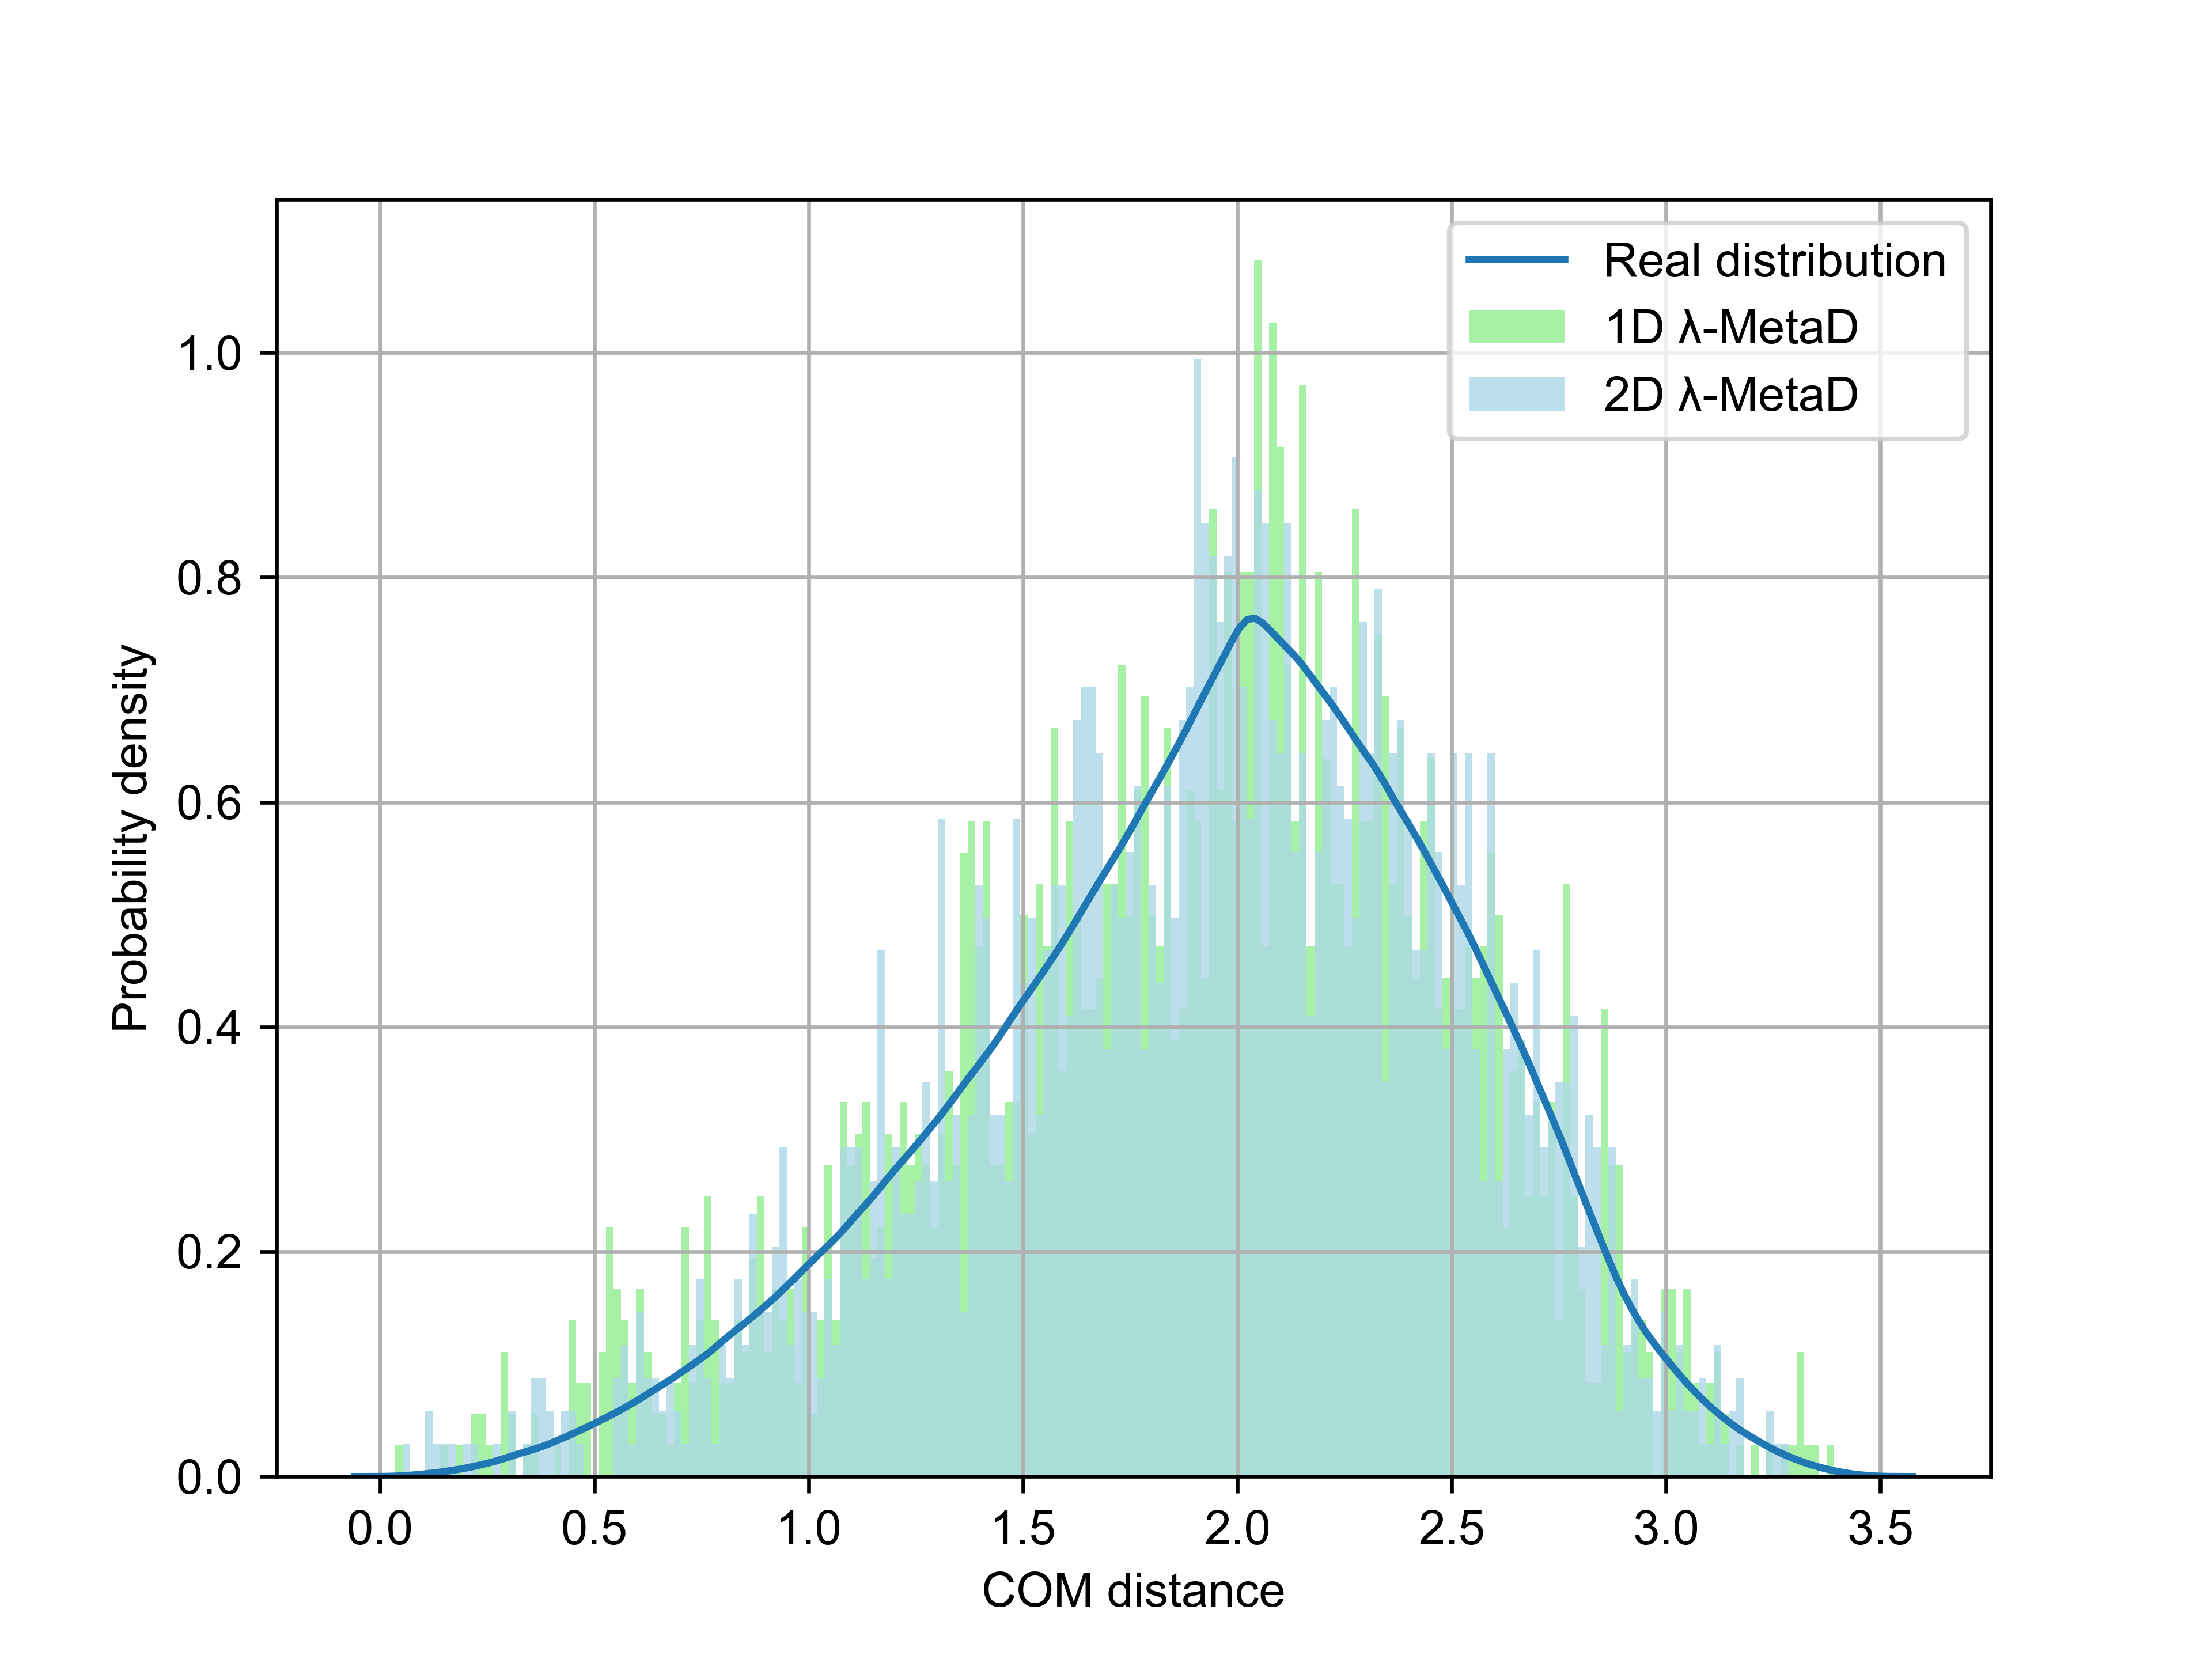
\includegraphics[width=0.7\textwidth]{Figures/pair_correlation_fitting}   
    \caption{The COM distance distributions obtained from the 1D and 2D alchemical metadynamics of System 3. The reference was an approximation to the real distribution by the distribution of the distance between the origin and each of the 5 million points randomly picked inside the simulation box.}
    \label{pair_correlation}
\end{figure}

\section{Standard MD simulations of System 3}
\subsection{time scale of water exclusion/inclusion}
In this section, we want to compare the time scales of water exclusion/inclusion of standard MD simulations with the one in the 1D alchemical metadynamics simulations as the complex simulation of System 3. The purpose of this comparison is to examine the degree of coupling between the alchemical variable and the number of water molecules in the binding cavity and to better understand how the water dynamics was changed under the influence of alchemical biases. To this end, we ran 10 standard MD simulations starting from 10 different fully coupled configurations with at least 9 water molecules in the binding cavity. These configurations were all drawn from the 1D alchemical metadynamics and they were considered as the unbound state of the binding complex. Each of the 10 simulations was performed for 200 ns in the NVT ensemble and they all used the same protocol adopted in the NVT equilibration during the preparation of Systems 1 or 2. 

As shown in Figure \ref{sys3_water_all}, the time scale of water exclusion can be anywhere between 10 ns and 125 ns, depending on how easy it was for the system to cross the free energy barrier from the starting configuration. On the other hand, after the host molecule was dehydrated, the system was generally trapped. This difference in the time scale between water exclusion (from large $N$ to small $N$) and inclusion (from small $N$ to large $N$) can be attributable to the difficulty levels of crossing the free energy barrier in different directions. Specifically, the 2D free energy surface in Figure 7 shows that in the fully coupled subspace, the bound state has a much lower free energy compared to the unbound state, so the transition from the dehydrated state back to the hydrated state was much harder than in the opposite direction. 

Interestingly, the time scale of water inclusion was significantly shortened in the 1D alchemical metadynamics (Figure 6) because the system was allowed to drift to other weakly-coupled states where the unbound state is generally more preferred. This shows that the alchemical variable is not significantly coupled to the number of water molecules in the binding cavity, which aligns with our intuition. Notably, the water exclusion was not necessarily accelerated in 1D alchemical metadynamics as compared to the standard MD simulations (Figure 6). This is because of the large free energy difference between the hydrated and dehydrated ends at higher alchemical states, which necessitates the introduction of the configurational bias in the 2D alchemical metadynamics detailed in the main text.

\begin{figure}[H]
    \centering
    \includegraphics[width=\textwidth]{Figures/sys3_water_all.png} 
    \caption{The time series of the number of water molecules obtianed from 10 standard MD simulations starting from the unbound state of the binding complex in System 3. }
    \label{sys3_water_all}
\end{figure}

\subsection{Estimation of the number of water molecules in the binding cavity of physical configurations}
As described in the main text, we used a switching function to estimate the number of water molecules in the binding cavity that replaced the space of the guest ligand. While the output of the switching function is constrained to be non-negative, it doesn't have natural or periodic boundaries. To prevent the configurational biases in 2D alchemical metadynamics from pushing the system to unphysical configurations that have excessive water molecules in the binding cavity, we set wall potentials as two cutoffs for setting the upper and lower bounds of the CV to discourage further sampling. Based on the 99.99 and 0.01 percentiles of the $N$ values in the time series obtained in the 10 standard MD simulations mentioned in the previous subsection, we set the cutoffs at $N=10.5$ and $N=0.7$. Notably, the two main purposes of the cutoffs are preventing computational resources to be wasted in sampling configurations we don't care about, and preventing any non-reversible changes such that the system can not return quickly to physical configurations. As long as the cutoffs could reach these two goals, their positions don't need to be precise since the biases from the wall potentials will be removed during reweighting as well.

% \clearpage
\section{Supplementary Figures}
\renewcommand{\thefigure}{S\arabic{figure}}
\begin{figure}[H]
    \centering
    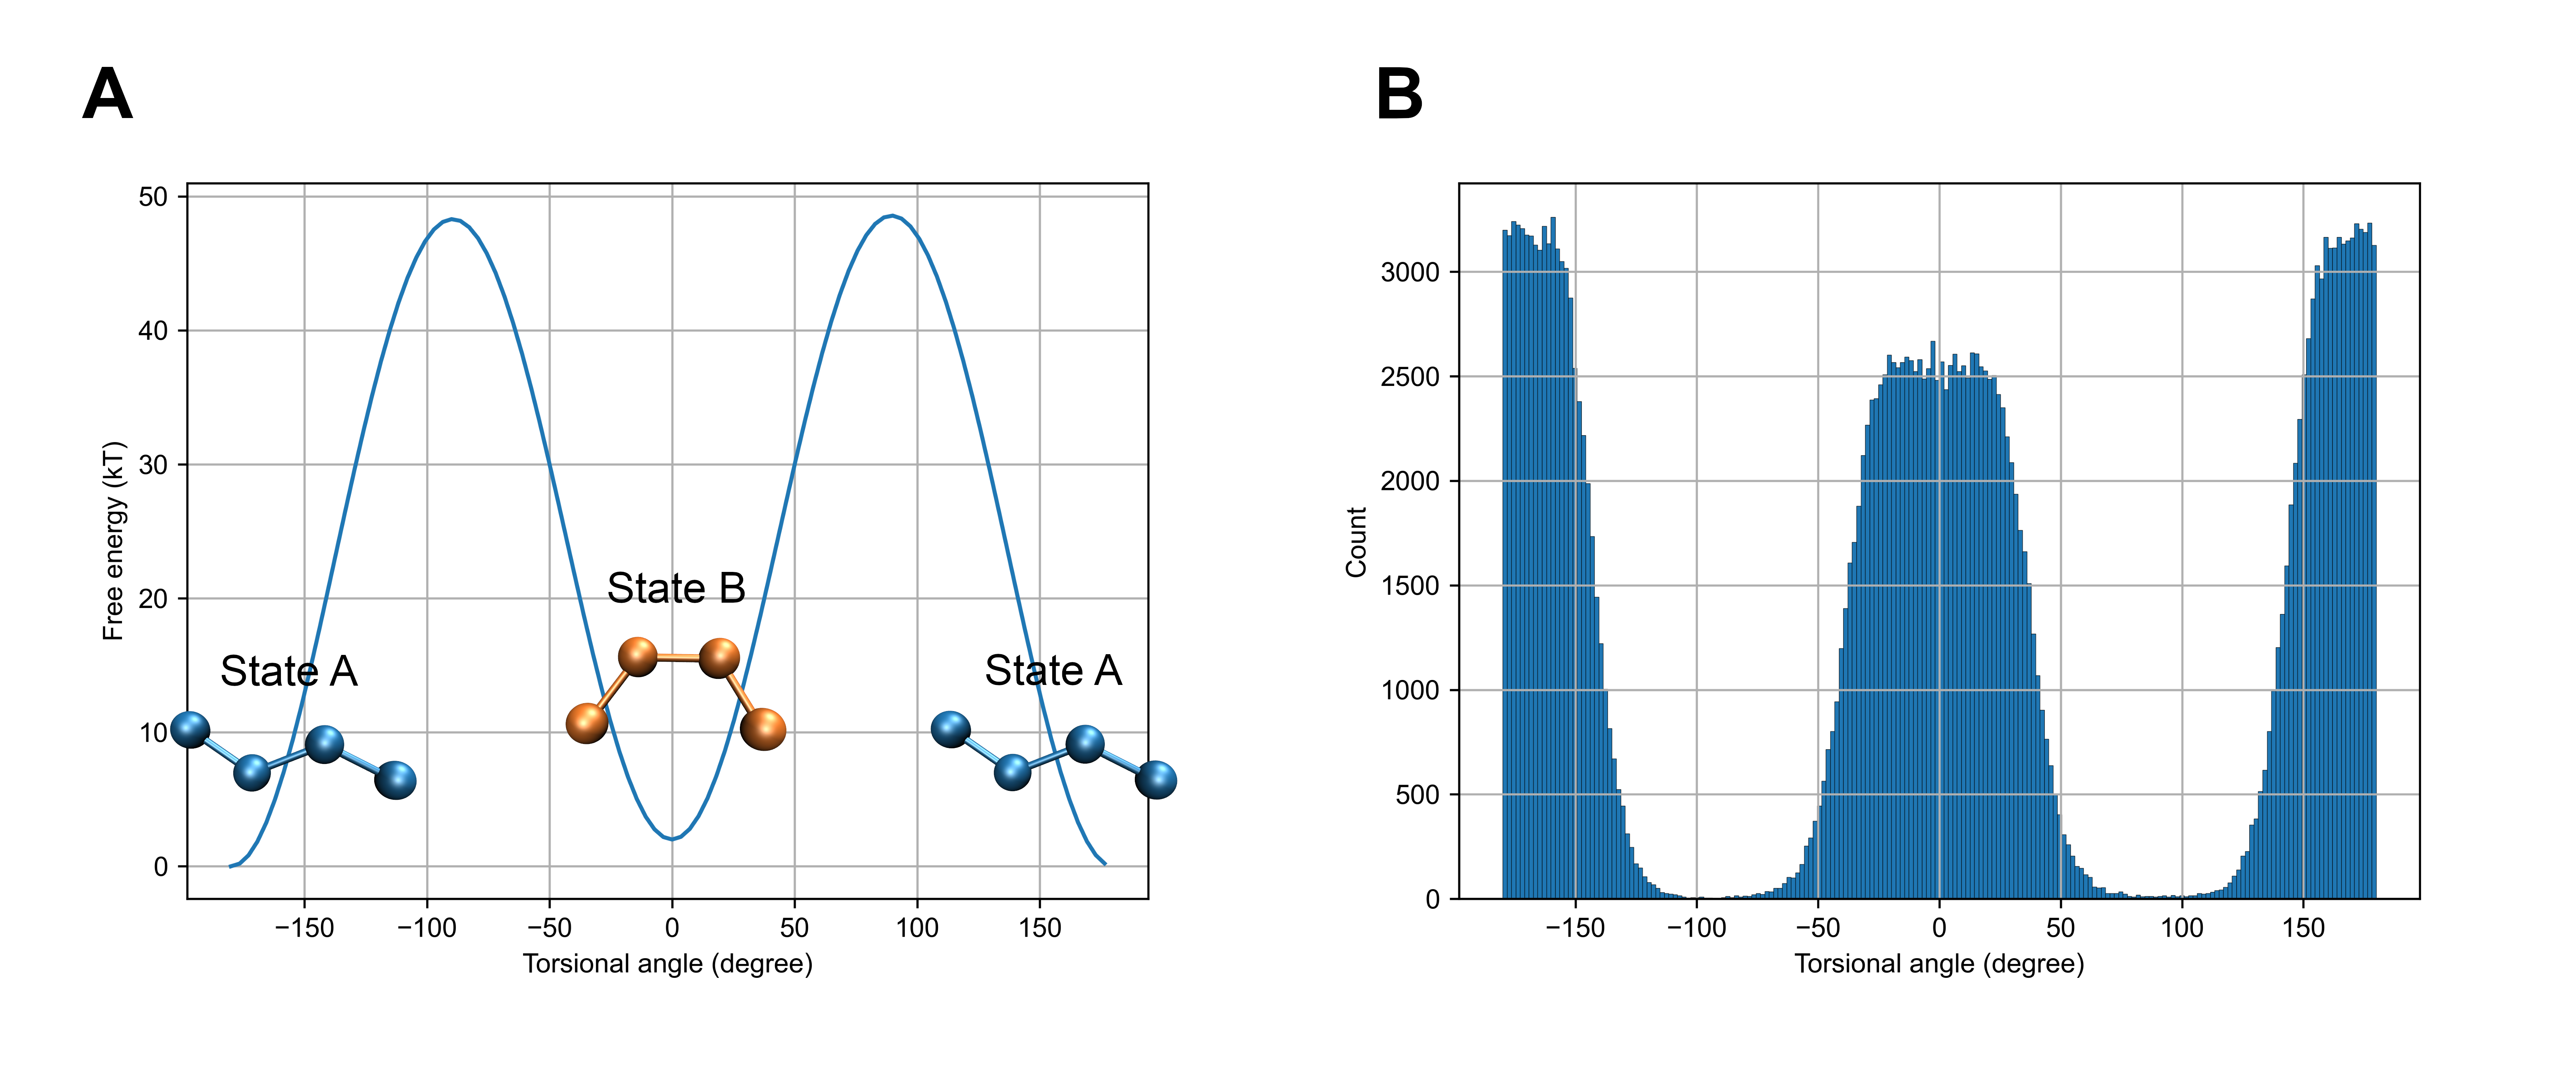
\includegraphics[width=\textwidth]{Figures/sys2_torsional_MetaD_annotated.png}   
    \caption{(A) The free energy profile as a function of the torsional angle. We refer the structures have a torsional angle of $\pm$180$^{\circ}$ and 0$^{\circ}$ as State A (trans isomer) and State B (cis isomer). The torsional free energy barrier starting from either state is around 48.56 kT, which might not be exact since the analysis was done on a very short (5 ns) simulation just for generating configurations at both states. (B) The histogram of the sampled torsional angle in the torsional metadynamics. As can be seen, the system was able to sample both states frequently during the short simulation.}
    \label{sys2_torsional_MetaD}
\end{figure}

\renewcommand{\thefigure}{S\arabic{figure}}
\begin{figure}[H]
    \centering
    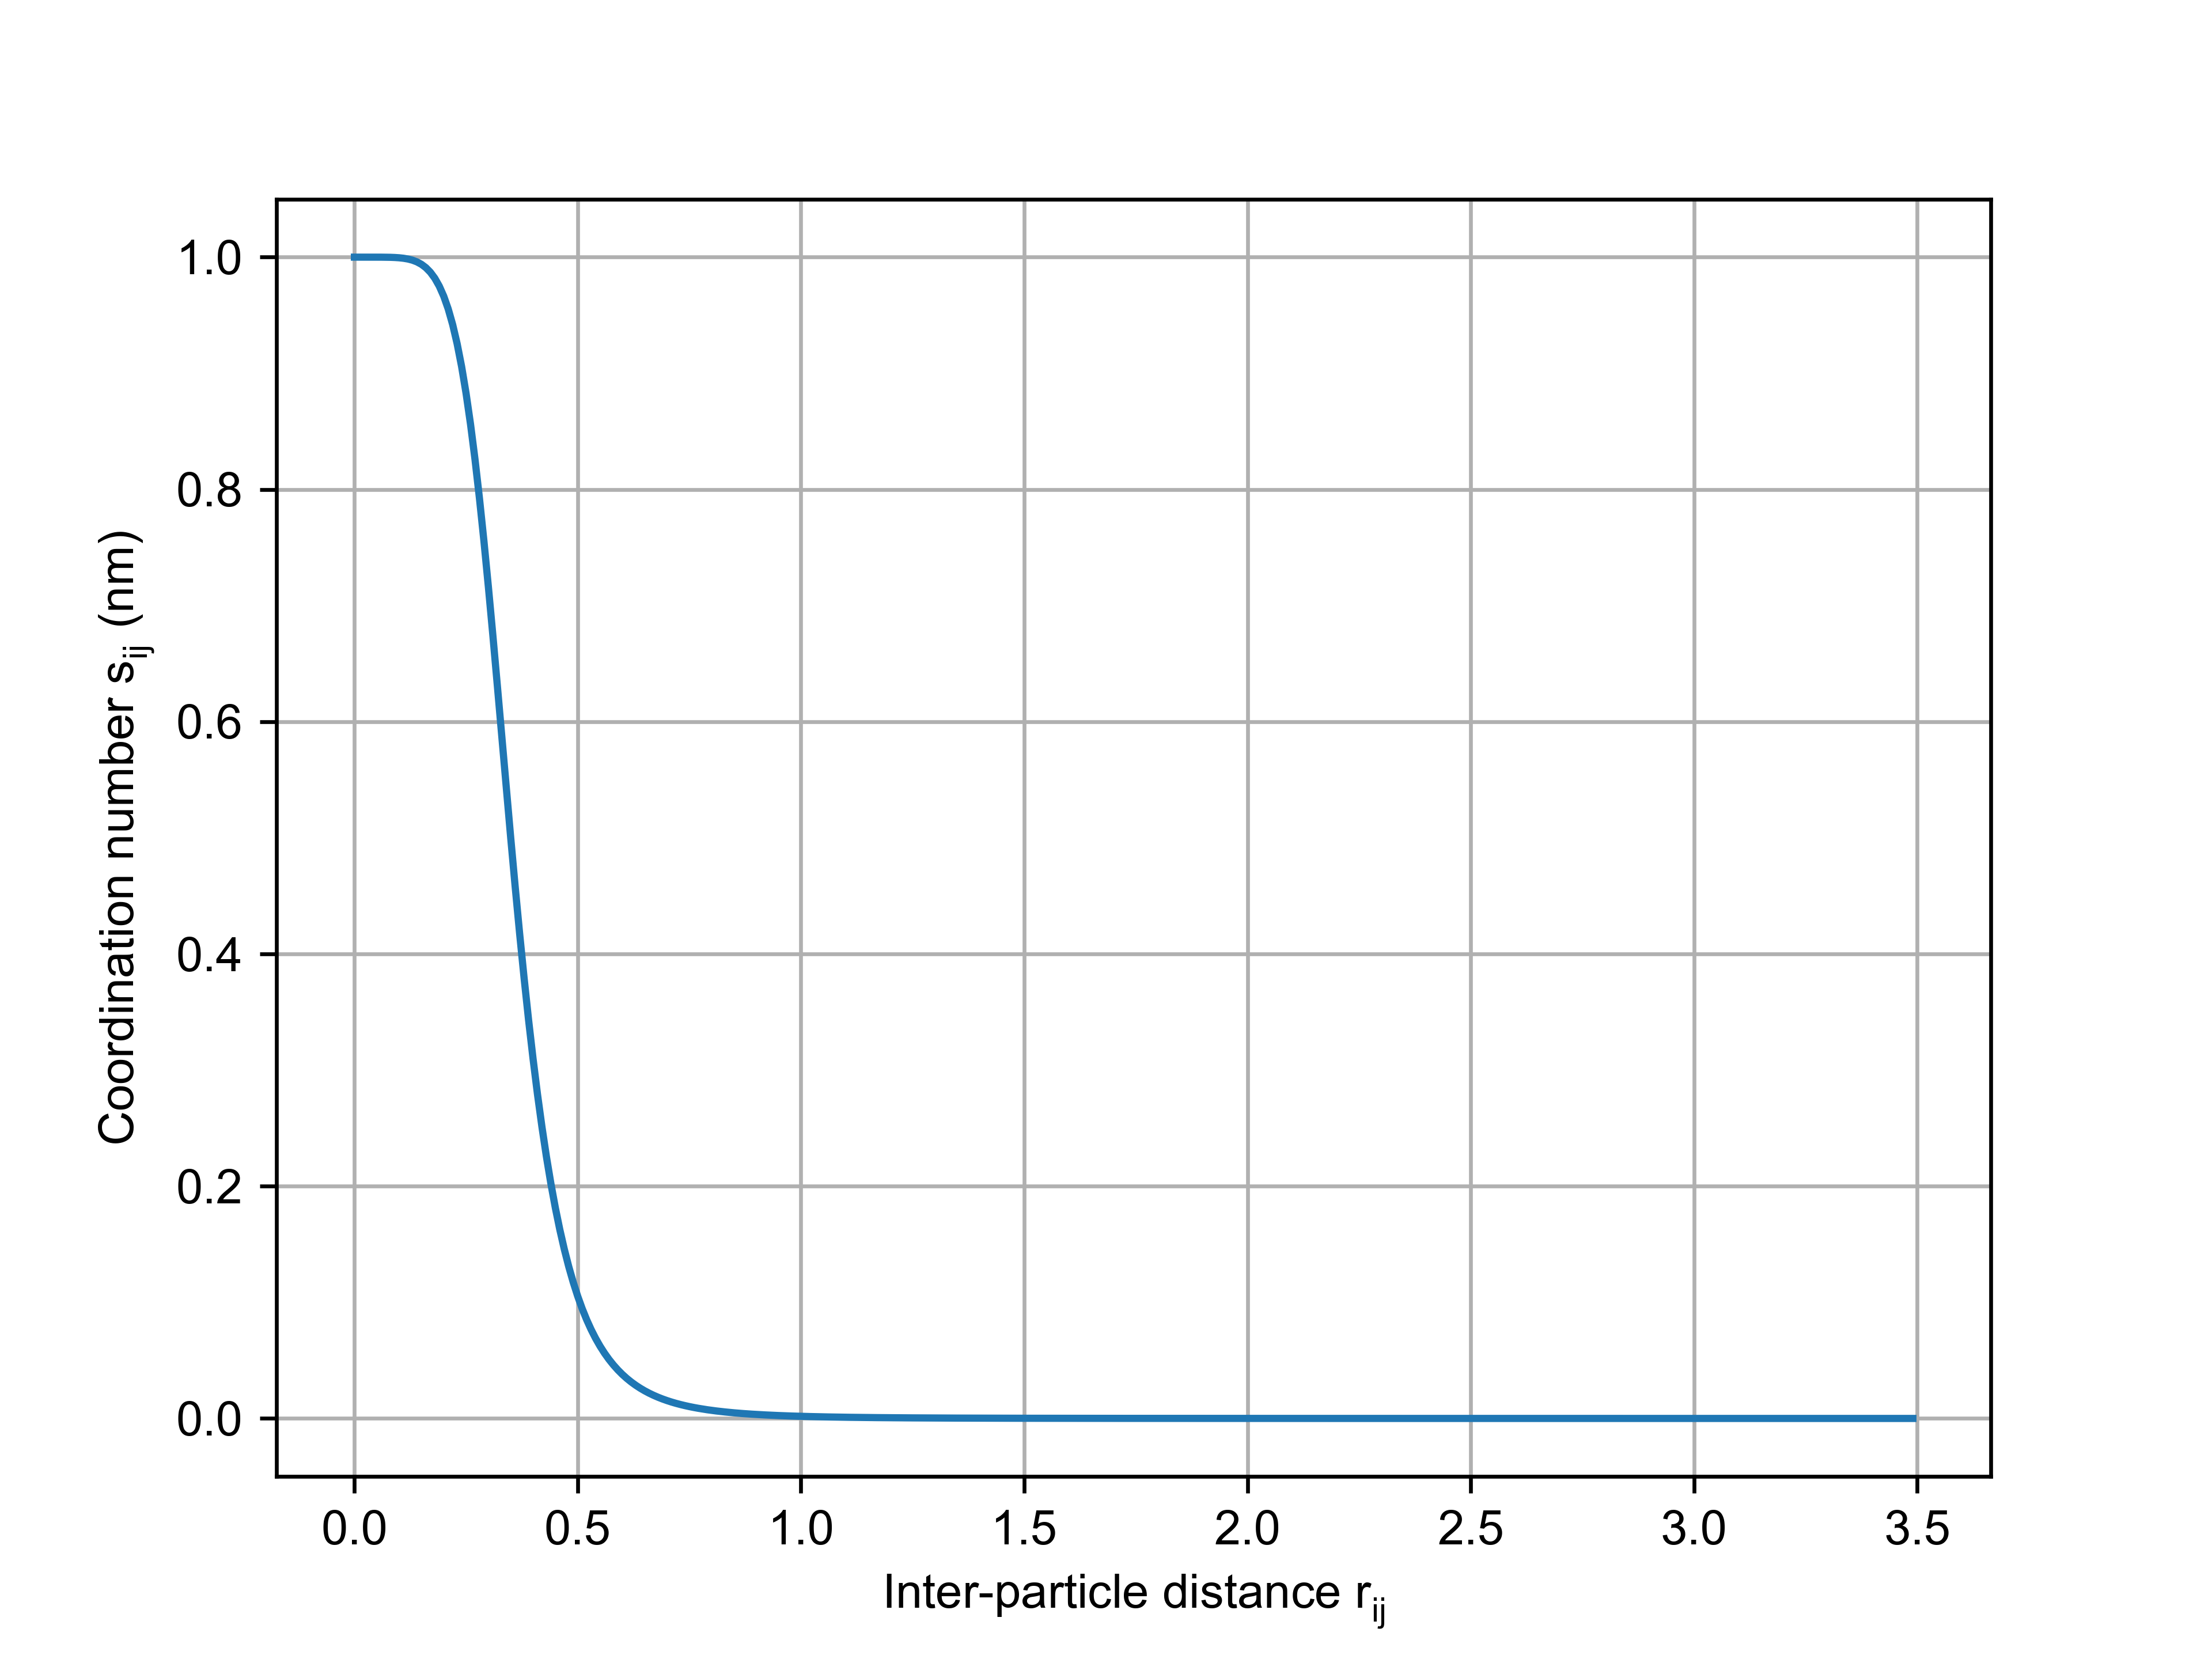
\includegraphics[width=0.7\textwidth]{Figures/switching_fn.png}   
    \caption{The switching function for estimating the coordination number between the host molecule atoms and the water molecules in System 3.}
    \label{switching}
\end{figure}

\renewcommand{\thefigure}{S\arabic{figure}}
\begin{figure}[H]
    \centering
    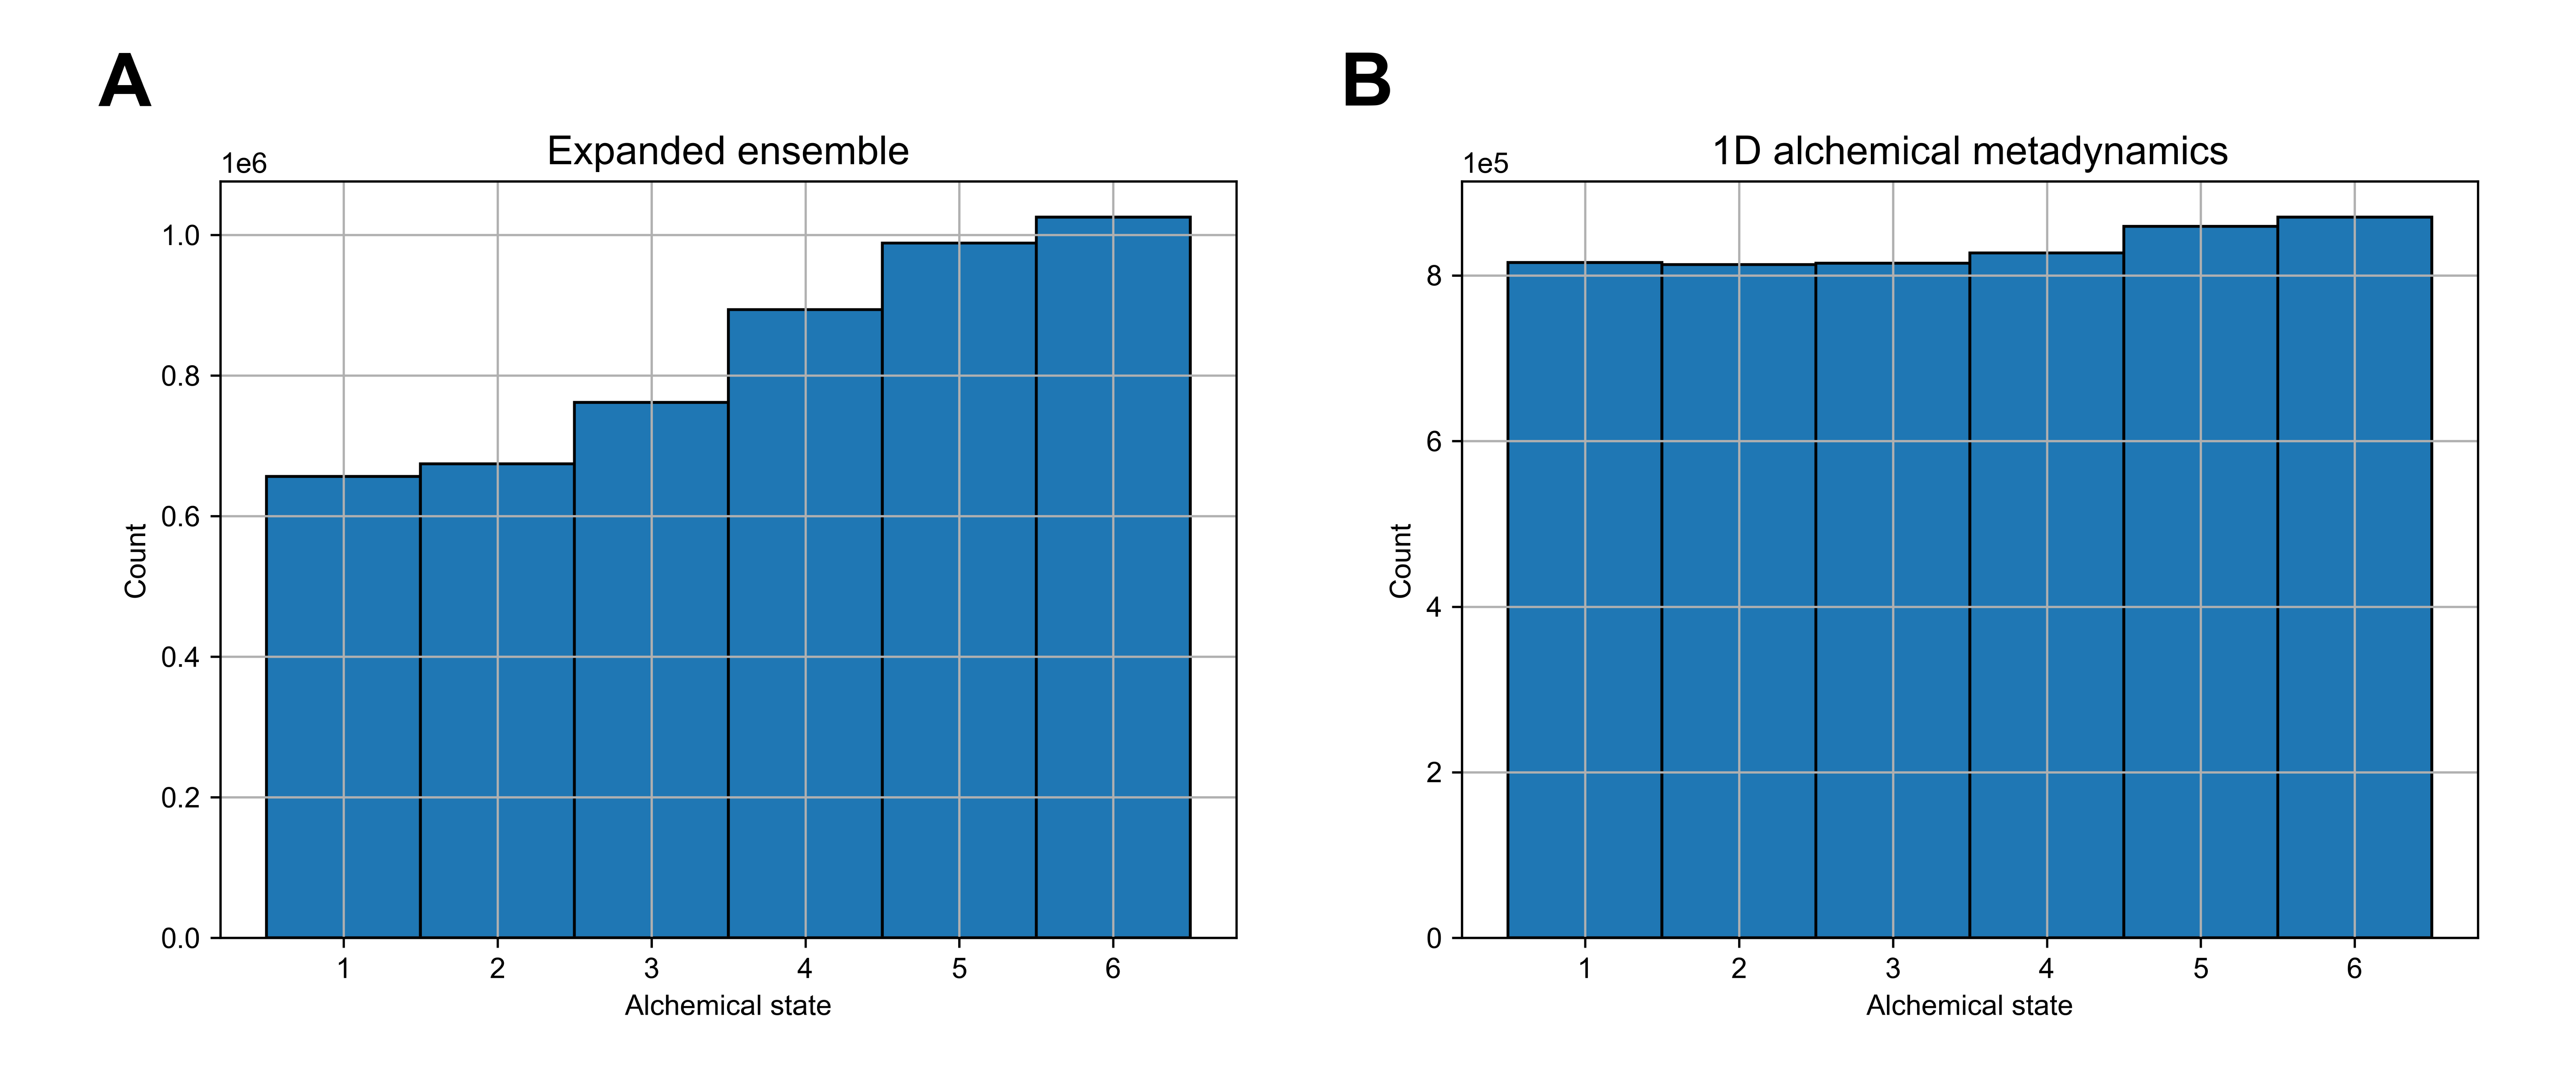
\includegraphics[width=\textwidth]{Figures/sys1_histograms.png}   
    \caption{The histograms of the state visitation in (A) expanded ensemble and (B) 1D alchemical metadynamics of System 1. Both simulations were able to sample all the intermediate states frequently.}
    \label{sys1_hist}
\end{figure}

\renewcommand{\thefigure}{S\arabic{figure}}
\begin{figure}[H]
    \centering
    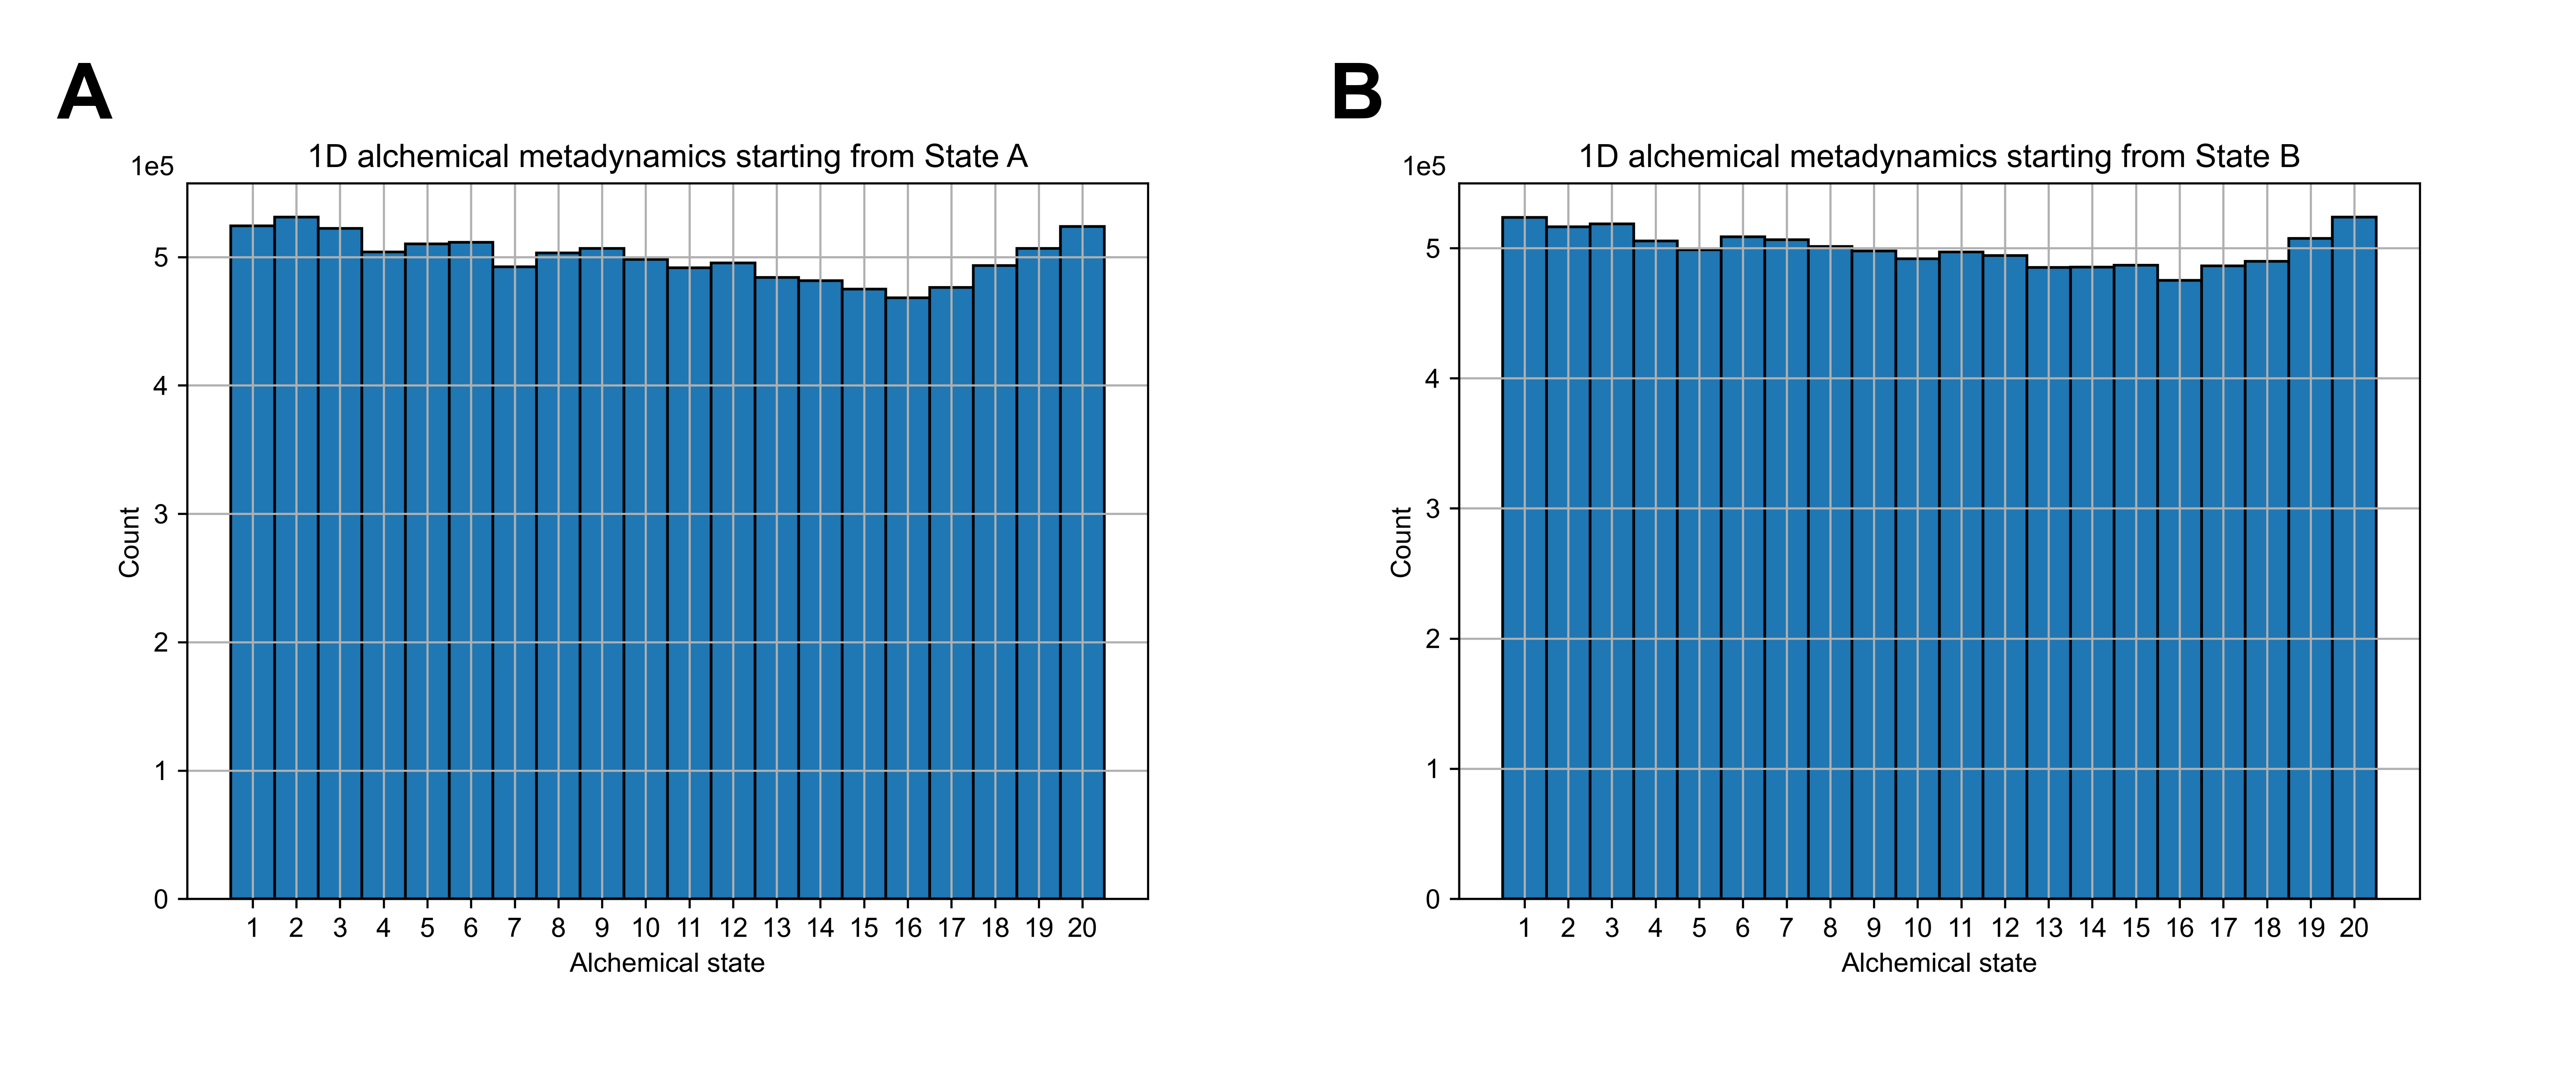
\includegraphics[width=\textwidth]{Figures/1D_lambda_hist.png}   
    \caption{The histograms of the state visitation in the 1D alchemical metadynamics starting from (A) State A and (B) State B. Both simulations were able to freely sample the alchemical space.}
    \label{sys2_1D_hist}
\end{figure}

\renewcommand{\thefigure}{S\arabic{figure}}
\begin{figure}[H]
    \centering
    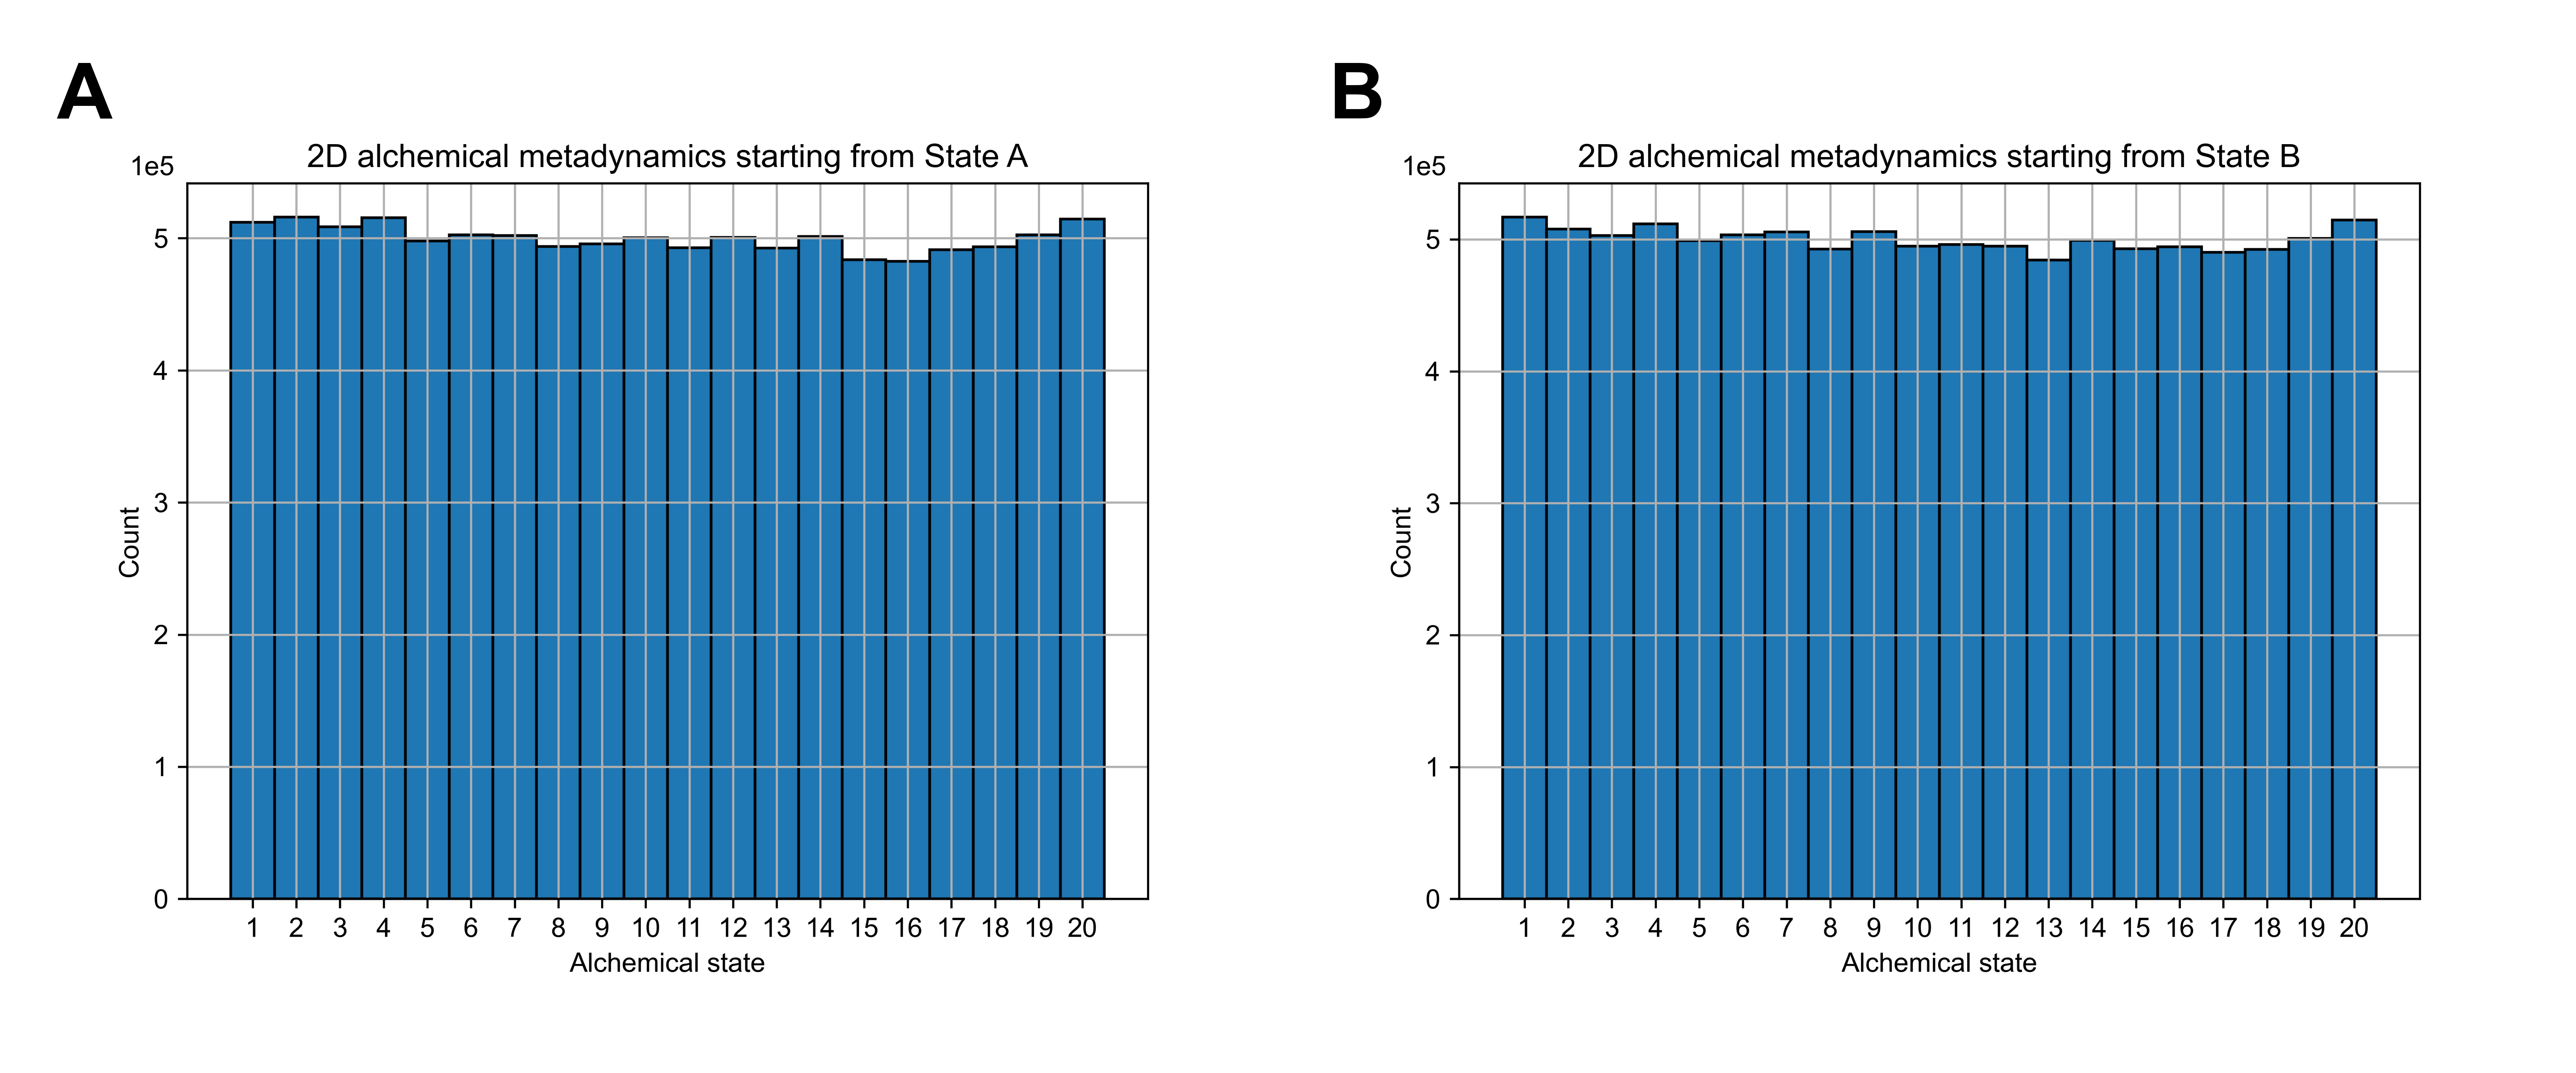
\includegraphics[width=\textwidth]{Figures/2D_lambda_hist.png}   
    \caption{The histograms of the state visitation in the 2D alchemical metadynamics starting from (A) State A and (B) State B. Similar to the two 1D simulations of System 2, both 2D simulations were able to freely sample the alchemical space.}
    \label{sys2_2D_hist}
\end{figure}

\renewcommand{\thefigure}{S\arabic{figure}}
\begin{figure}[H]
    \centering
    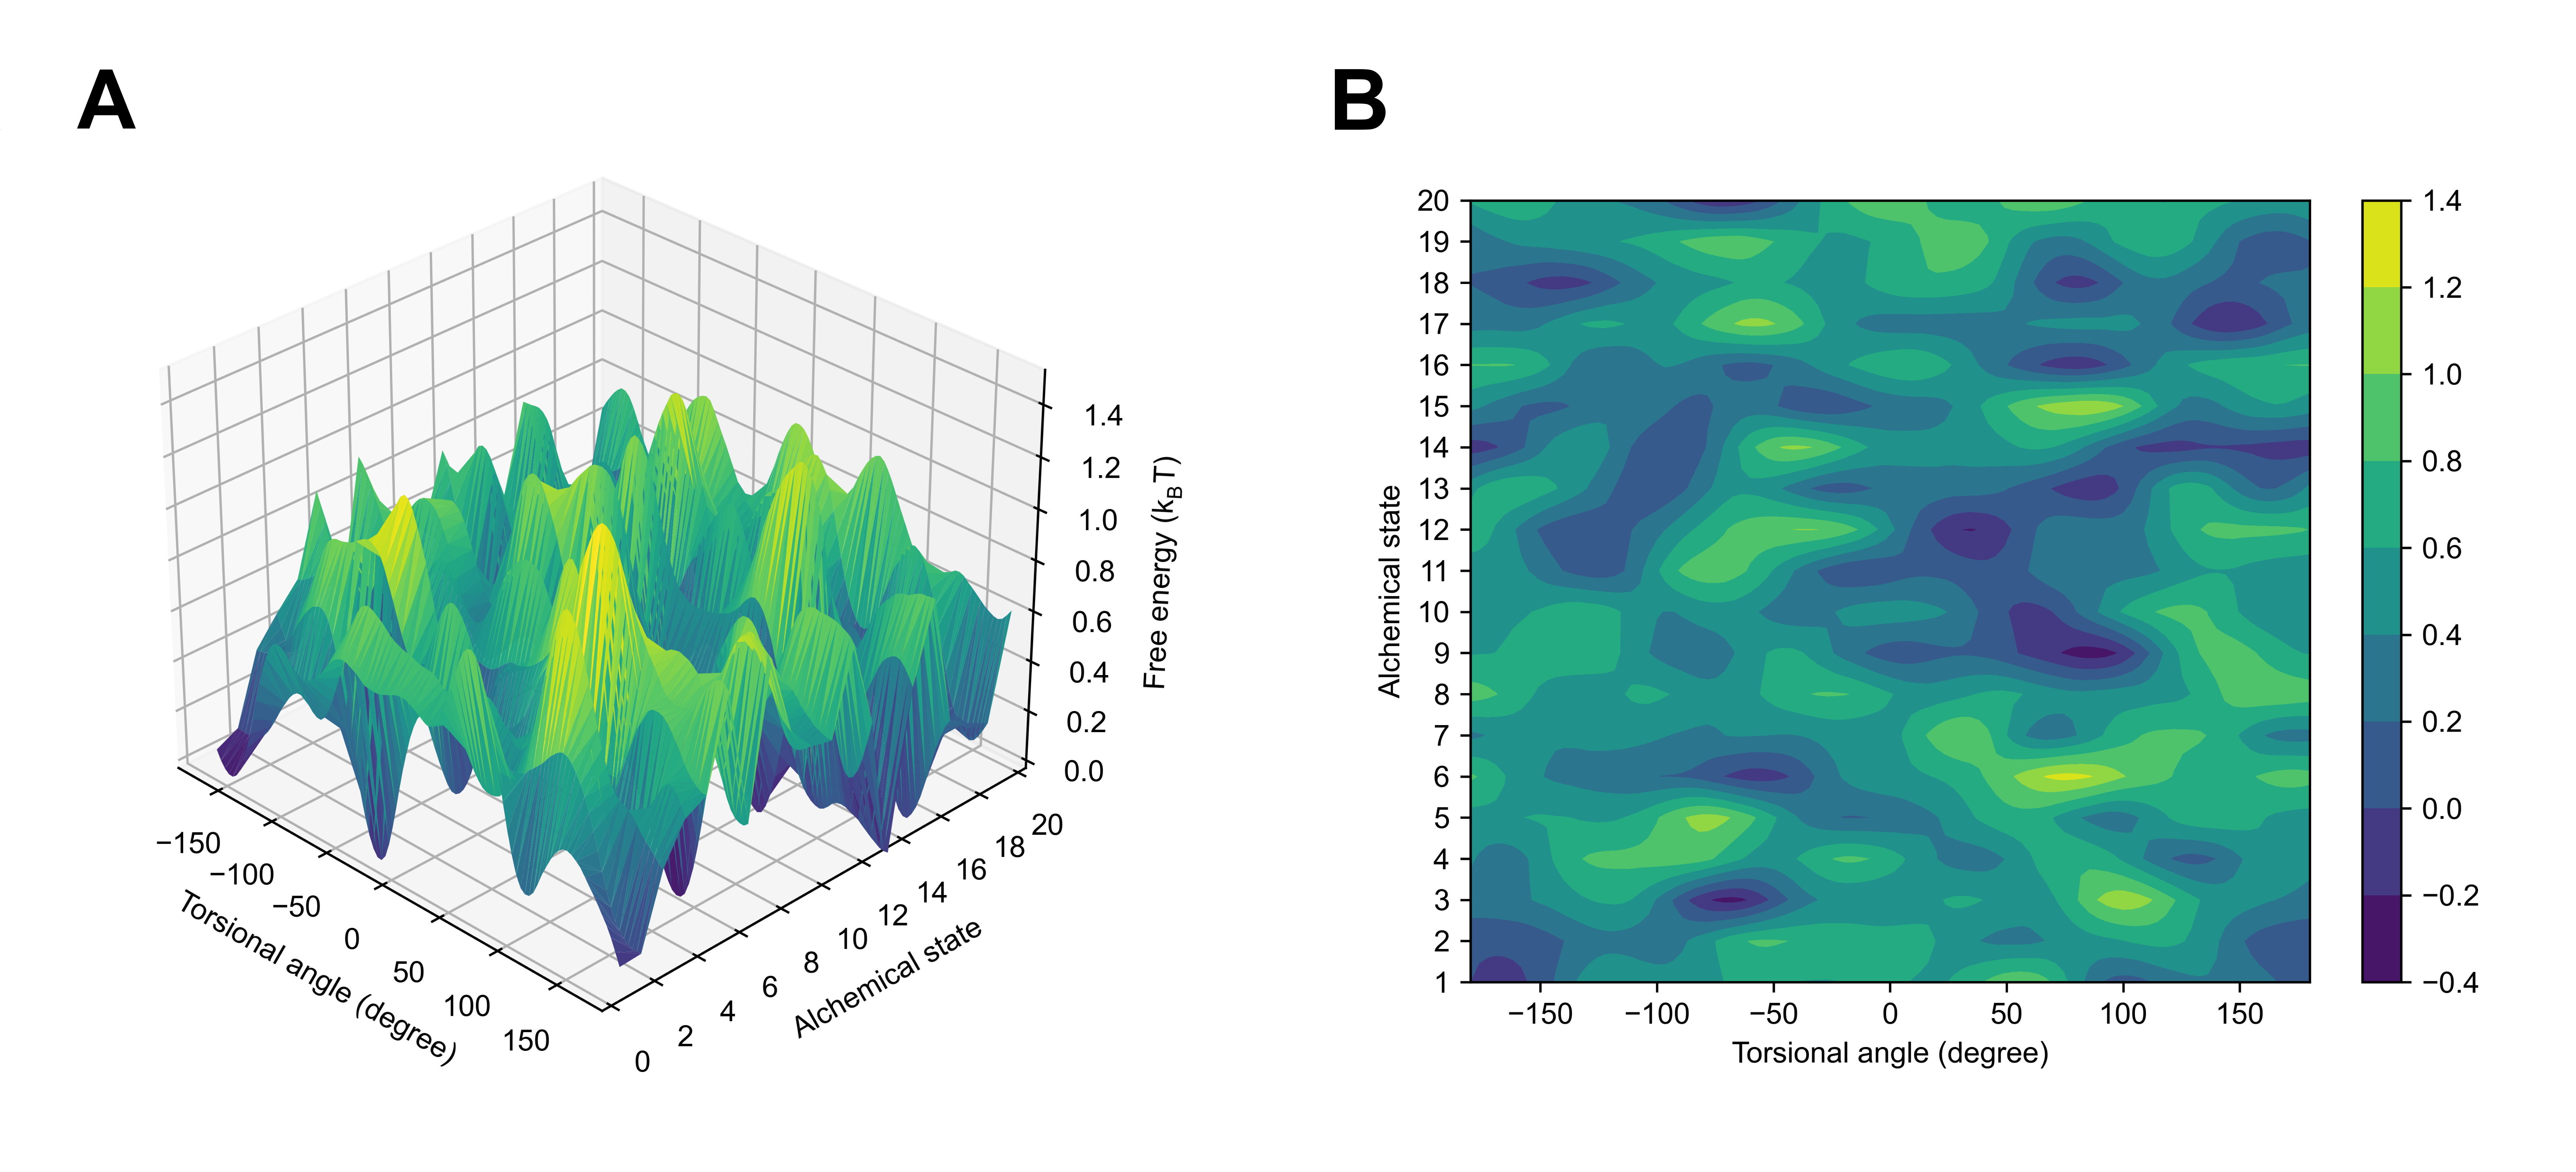
\includegraphics[width=\textwidth]{Figures/sys2_fes_contour_diff_annotated.png}   
    \caption{(A) The difference between the free energy surfaces and (B) the difference between contour plots obtained from the two 2D alchemical metadynamics simulations of System 2.}
    \label{sys2_fes_diff}
\end{figure}

\renewcommand{\thefigure}{S\arabic{figure}}
\begin{figure}[H]
    \centering
    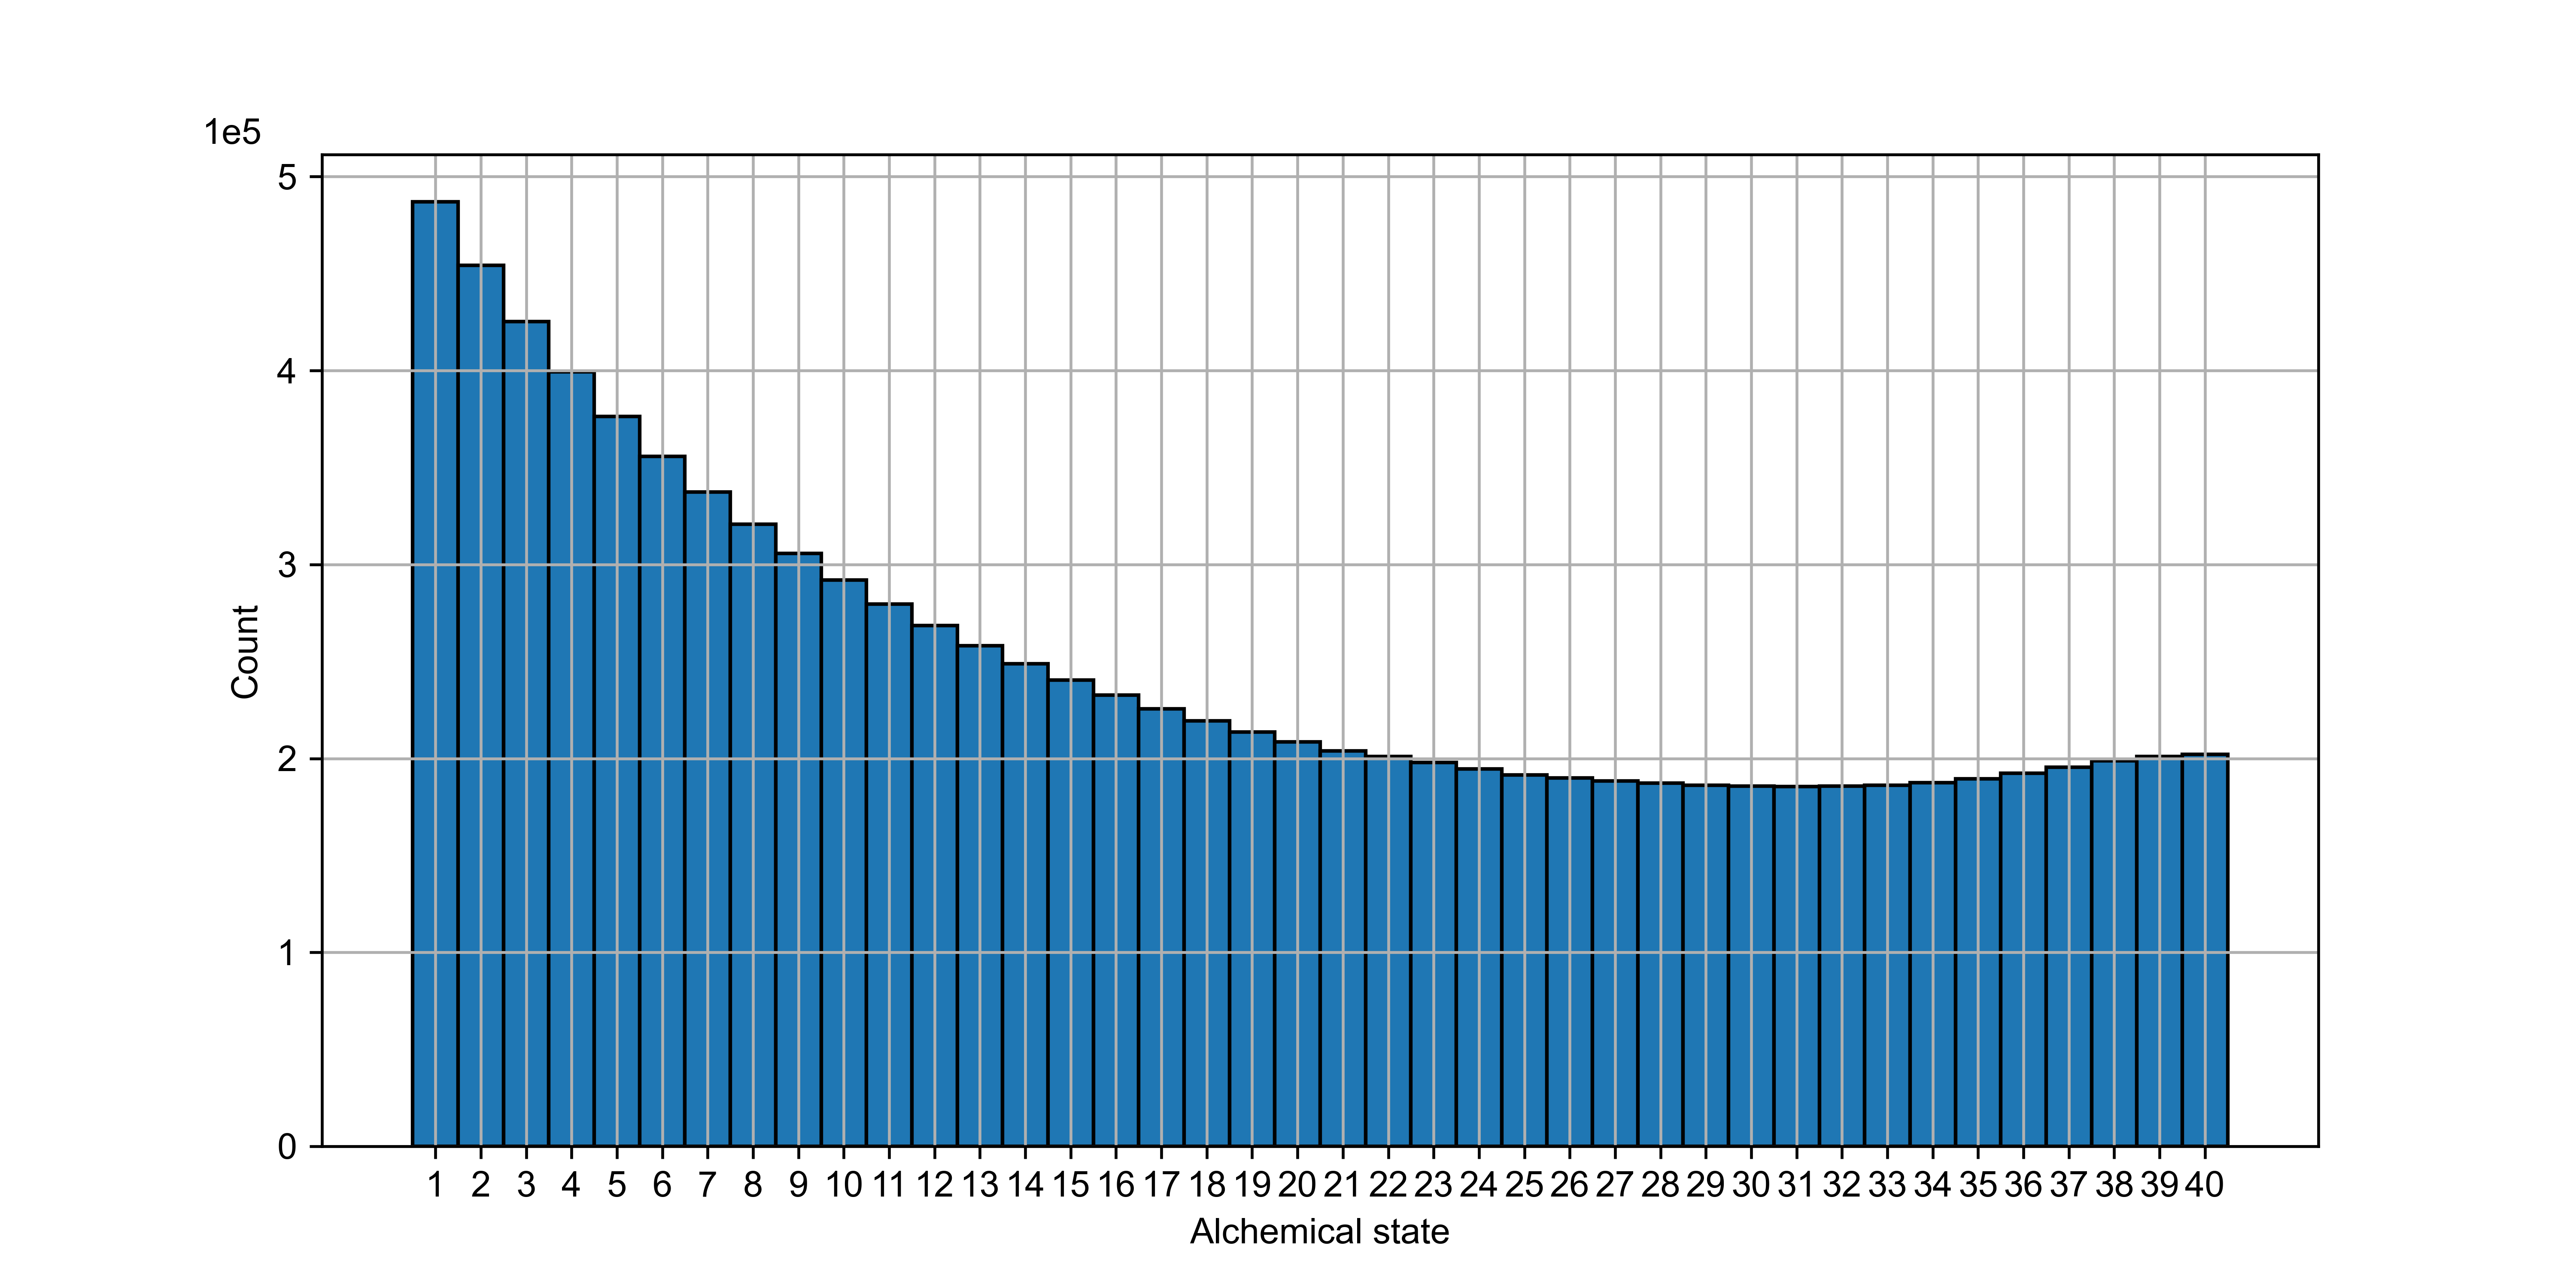
\includegraphics[width=\textwidth]{Figures/lambda_hist.png}   
    \caption{The histograms of the state visitation in the 1D alchemical metadynamics as the solvent simulation of System 3. The system was able to sample all the alchemical intermediate states frequently.}
    \label{sys3_1D_hist}
\end{figure}


\clearpage
\bibliography{refs}

\end{document}